\documentclass{article}
\usepackage{ae,aecompl}
\usepackage{todonotes}
\usepackage{chngcntr}
\usepackage{tikz-cd}
\usepackage{graphicx}
\graphicspath{ {./images/}}
\usepackage[all,cmtip]{xy}
\usepackage{amsmath, amscd}
\usepackage{amsthm}
\usepackage{amssymb}
\usepackage{amsfonts}
\usepackage{bm}
\usepackage{qsymbols}
\usepackage{latexsym}
\usepackage{mathrsfs}
\usepackage{mathtools}
\usepackage{cite}
\usepackage{color}
\usepackage{url}
\usepackage{enumerate}
\usepackage{verbatim}
\usepackage[draft=false, colorlinks=true]{hyperref}
\usepackage{pdfpages}
\usepackage[margin=1.2in]{geometry}
\usepackage{IEEEtrantools}

\usepackage{fancyhdr}


\usepackage[nameinlink]{cleveref}


\DeclareMathOperator*{\ac}{accept}
\DeclareMathOperator*{\amax}{argmax}
\DeclareMathOperator*{\amin}{argmin}
\DeclareMathOperator*{\Aut}{Aut}
\newcommand {\al}{{\alpha}}
\newcommand {\abs}[1]{{\left\lvert#1\right\rvert}}
\newcommand {\A}{{\mathcal{A}}}
\newcommand {\AM}{{\mathrm{AM}}}
\newcommand {\AMp}{{\AM_{p}^{X}\!(\Ri_\w)}}
\newcommand {\B}{{\mathcal{B}}}
\DeclareMathOperator*{\Be}{Bern}
\newcommand {\Br}{{\dot{B}}}
\newcommand {\Ba}{{\mathfrak{B}}}
\newcommand {\C}{{\mathbb C}}
\newcommand {\ce}{\mathrm{c}}
\newcommand {\Ce}{\mathrm{C}}
\newcommand {\Cc}{\mathrm{C_{c}}}
\newcommand {\Ccinf}{\mathrm{C_{c}^{\infty}}}
\DeclareMathOperator{\cov}{Cov}
\DeclareMathOperator{\DEV}{DEV}
\newcommand {\Di}{{\mathbb D}}
\newcommand {\dom}{\mathrm{dom}}
\newcommand{\dist}{\stackrel{\mathrm{dist}}{=}}
\newcommand {\ud}{\mathrm{d}}
\newcommand {\ue}{\mathrm{e}}
\newcommand {\eps}{\varepsilon}
\newcommand {\veps}{\varepsilon}
\newcommand {\vrho}{{\varrho}}
\newcommand {\E}{{\mathbb{E}}}
\newcommand {\Ec}{{\mathcal{E}}}
\newcommand {\Ell}{L}
\newcommand {\Ellp}{{L_{p}[0,1]}}
\newcommand {\Ellpprime}{{L_{p'}([0,1])}}
\newcommand {\Ellq}{{L_{q}([0,1])}}
\newcommand {\Ellqprime}{{L_{q'}([0,1])}}
\newcommand {\Ellr}{L^{r}}
\newcommand {\Ellone}{{L_{1}([0,1])}}
\newcommand{\Elltwo}{{L_{2}([0,1])}}
\newcommand{\Ellinfty}{L^{\infty}}
\newcommand{\Ellinftyc}{L_{\mathrm{c}}^{\infty}}
\newcommand{\exb}[1]{\exp\left\{#1\right\}}
\DeclareMathOperator*{\Ext}{Ext}
\newcommand{\F}{{\mathcal{F}}}
\newcommand{\Fe}{{\mathbb{F}}}
\newcommand{\G}{{\mathcal{G}}}
\newcommand{\HF}{\mathcal{H}_{\text{FIO}}^{1}(\Rd)}
\newcommand{\Hr}{H}
\newcommand{\HT}{\mathcal{H}}
\newcommand{\ui}{\mathrm{i}}
\newcommand{\I}{{I}}
\newcommand{\J}{{\mathcal{J}}}
\newcommand{\id}{{\mathrm{id}}}
\newcommand{\iid}{\stackrel{\mathclap{\normalfont\mbox{iid}}}{\sim}}
\newcommand{\im}{{\text{im }}}
\newcommand{\ind}{{\perp\!\!\!\perp}}
\DeclareMathOperator*{\Int}{int}
\newcommand{\intx}{{\overline{\int_{X}}}}
\newcommand{\inte}{{\overline{\int_{\E}}}}
\newcommand{\la}{\lambda}
\newcommand{\rb}{\rangle}
\newcommand{\lb}{{\langle}}
\newcommand{\La}{\Lambda}
\newcommand{\calL}{{\mathcal{L}}}
\newcommand{\lp}{{\mathcal{L}}^{p}}
\newcommand{\lpo}{{\overline{\mathcal{L}}^{p}\!}}
\newcommand{\Lpo}{{\overline{\Ell}^{p}\!}}
\newcommand{\M}{{\mathbf{M}}}
\newcommand{\Ma}{{\mathcal{M}}}
\newcommand{\N}{{{\mathbb N}}}
\newcommand{\Na}{{{\mathcal{N}}}}
\newcommand{\norm}[1]{\left\|#1\right\|}
\newcommand{\normm}[1]{{\left\vert\kern-0.25ex\left\vert\kern-0.25ex\left\vert #1 
    \right\vert\kern-0.25ex\right\vert\kern-0.25ex\right\vert}}
\newcommand{\Om}{{{\Omega}}}
\newcommand{\one}{{{\bf 1}}}
\newcommand{\pic}{\text{Pic }}
\newcommand{\ph}{{\varphi}}
\newcommand{\Pa}{{\mathbb{P}}}
\newcommand{\Po}{{\mathcal{P}}}
\newcommand{\Q}{{\mathbb{Q}}}
\newcommand{\R}{{\mathbb R}}
\newcommand{\Rd}{{\mathbb{R}^{d}}}
\DeclareMathOperator{\rej}{reject }
\newcommand{\Rn}{{\mathbb{R}^{n}}}
\newcommand{\cR}{{\mathcal{R}}}
\newcommand{\Rad}{{\mathrm{Rad}}}
\newcommand{\ran}{{\mathrm{ran}}}
\newcommand{\Ri}{{\mathrm{R}}}
\newcommand{\supp}{{\mathrm{supp}}}
\newcommand{\Se}{\mathrm{S}}
\newcommand{\Sp}{S^{*}(\Rn)}
\newcommand{\St}{{\mathrm{St}}}
\newcommand{\Sw}{\mathcal{S}}
\newcommand{\T}{{\mathcal{T}}}
\newcommand{\ta}{{\theta}}
\newcommand{\Ta}{{\Theta}}
\newcommand{\topp}{\stackrel{p}{\to}}
\newcommand{\todd}{\stackrel{d}{\to}}
\newcommand{\toL}[1]{\stackrel{L^{#1}}{\to}} 
\newcommand{\toas}{\stackrel{a.s.}{\to}}
\DeclareMathOperator{\V}{Var}
\newcommand {\w}{{\omega}}
\newcommand {\W}{{\mathrm{W}}}
\newcommand {\Wnp}{\text{$\mathrm{W}$\textsuperscript{$n,\!p$}}}
\newcommand {\Wnpeq}{\text{$\mathrm{W}$\textsuperscript{$n\!,\!p$}}}
\newcommand {\Wonep}{\text{$\mathrm{W}$\textsuperscript{$1,\!p$}}}
\newcommand {\Wonepeq}{\text{$\mathrm{W}$\textsuperscript{$1\!,\!p$}}}
\newcommand {\X}{{\mathcal{X}}}
\newcommand {\Z}{{{\mathbb Z}}}
\newcommand {\Za}{{\mathcal{Z}}}
\newcommand {\Zd}{{\Z[\sqrt{d}]}}
\newcommand {\vanish}[1]{\relax}

\newcommand {\wh}{\widehat}
\newcommand {\wt}{\widetilde}
\newcommand {\red}{\color{red}}

% Distributions
\newcommand{\normal}{\mathsf{N}}
\newcommand{\poi}{\mathsf{Poisson}}
\newcommand{\bern}{\mathsf{Bernoulli}}
\newcommand{\bin}{\mathsf{Binomal}}
\newcommand{\multi}{\mathsf{Multinomial}}
\newcommand{\Exp}{\mathsf{Exp}}



% put your command and environment definitions here




% some theorem environments
% remove "[theorem]" if you do not want them to use the same number sequence


  \newtheorem{thrm}{Theorem}
  \newtheorem{lemma}{Lemma}
  \newtheorem{prop}{Proposition}
  \newtheorem{cor}{Corollary}

  \newtheorem{conj}{Conjecture}
  \renewcommand{\theconj}{\Alph{conj}}  % numbered A, B, C etc

  \theoremstyle{definition}
  \newtheorem{defn}{Definition}
  \newtheorem{ex}{Example}
  \newtheorem{exs}{Examples}
  \newtheorem{question}{Question}
  \newtheorem{remark}{Remark}
  \newtheorem{notn}{Notation}
  \newtheorem{exer}{Exercise}




\title{STATS305A - Lecture 16}
\author{John Duchi\\ Scribed by Michael Howes}
\date{11/16/21}

\pagestyle{fancy}
\fancyhf{}
\rhead{STATS305A - Lecture 16}
\lhead{11/16/21}
\rfoot{Page \thepage}

\begin{document}
\maketitle
\tableofcontents
\section{Announcements}
\begin{itemize}
    \item HW3 due Friday.
    \item Etude 3 due Friday and corrections due Monday.
\end{itemize}
Today we will be discussing two randomized methods - cross validation and permutation tests.

\section{Validation}
Suppose we have a fitting method $\wh{\beta}$. We'd like to know how $\wh{\beta}$ is going perform on future data. In a typical case we would have a hyperparameter $\la$ and we want to pick the ``best'' $\la$. We have seen many examples of different things $\la$ could represent, such as:

\begin{itemize}
    \item We could have $\la$ equal to the regularization parameter in ridge regression.
    \item We could also have $\la$ equal to the number of coordinates in PC regression, forward stepwise regression or boosting.
\end{itemize}
Define 
\[R(b) = \E[L(Y_{n+1}, X_{n+1}^Tb)],\]
for some loss function $L : \R \times \R \to \R$. The quantity $R(b)$ is the out-of-sample risk of the linear predictor $\wh{y}= x^Tb$. We wish to estimate $R(b)$ and choose $\la$ which minimizes $R(\wh{\beta})$. There are two approaches that we will discuss, using a hold out set or performing cross validation.
\subsection{Hold out set}
Hold out a subset of our data, call it the \emph{validation data}. Fit the model on \emph{training data} (which is all the data apart from the validation set). We can the calculate the average loss on the independent validation set. There are two issues with this
\begin{itemize}
    \item It can be a little high variance.
    \item We are not using all the data.
\end{itemize}
\subsection{Cross validation}
The idea behind cross validation is to split our data into $k$ equal sized partitions which we call \emph{folds}. For each fold we fit on the remaining $k-1$ folds and then evaluate the model on the held out fold. 

More mathematically, let $J(i)$ be the set of indices in fold $i$. Define
\[\wh{\beta}^{-J(i)} = \text{model fit on $(X,Y)$ but with the indices in $J(i)$ removed.}\]
The emperical risk of using a linear predictor $b$ on fold $i$ is
\[\wh{R}_i(b) =\frac{1}{\abs{J(i)}}\sum_{i \in J(i)} L(y_j, x_j^Tb),\]
where $\abs{J(i)}$ is the cardinality of $J(i)$ which is typically $\frac{n}{k}$ (this happens when all the folds are the exact same size). Then define the $k$-fold cross validation error to be
\[CV(k) = \frac{1}{k} \sum_{i=1}^k \wh{R}_i(\wh{\beta}^{-J(i)}). \]
Two natural questions are:
\begin{enumerate}
    \item What is $CV(k)$ approximating?
    \item What do we use $CV(k)$ for?
\end{enumerate}
Let $\T$ be a training set $(X,Y) \in \R^{n \times d} \times \R^n$. What we'd like to know is
\[\text{Err}(\T) = R(\wh{\beta}(\T)),\]
where $\wh{\beta}(\T)$ is the model trained using our test set $\T$. We'd like to know the expected error of using $\wh{\beta}(\T)$ on new data. Our training set is considered to be random and thus we can define
\[ \text{Err}_n = \E[\text{Err}(\T)],\]
where the expectation is taken over all training sets of size $n$. If we assume that our data is i.i.d. and the $k$ folds all have size $\frac{n}{k}$, then
\begin{align*}
    \E[CV(k)]&=\E[\wh{R}_k(\wh{\beta}^{-J(k)})]\\
    &=\E\left[\E\left[\wh{R}_k(\wh{\beta}^{-J(k)})\middle|-J(k)\right] \right]\\
    &=\E[R(\wh{\beta}(\text{training set of size } n-k/n))]\\
    &=\text{Err}_{\frac{(k-1)n}{k}}+
\end{align*}
Thus we have an issue $\E[CV(k)]$ is not unbiased for $\text{Err}_n$. There are some ``solutions''
\begin{itemize}
    \item Just ignore the bias.
    \item Introduce correction terms. These can be a bit complicated and will depend on the loss function $L$ and the choice of model fitting procedure. See John's notes for some details in special cases.
    \item If we take $k$ large, $\text{Err}_{\frac{(k-1)n}{k}}$ will be close to $n$. We will discuss this more in the leave one out section.
\end{itemize}
\subsection{Using cross validation for model selection}
In partice we calculate $CV(k)$ for various values of $\la$ and then compare $CV(k)$ accross these values. If we plot $CV(k)$ we tend to see pictures that look like this:

\begin{center}
    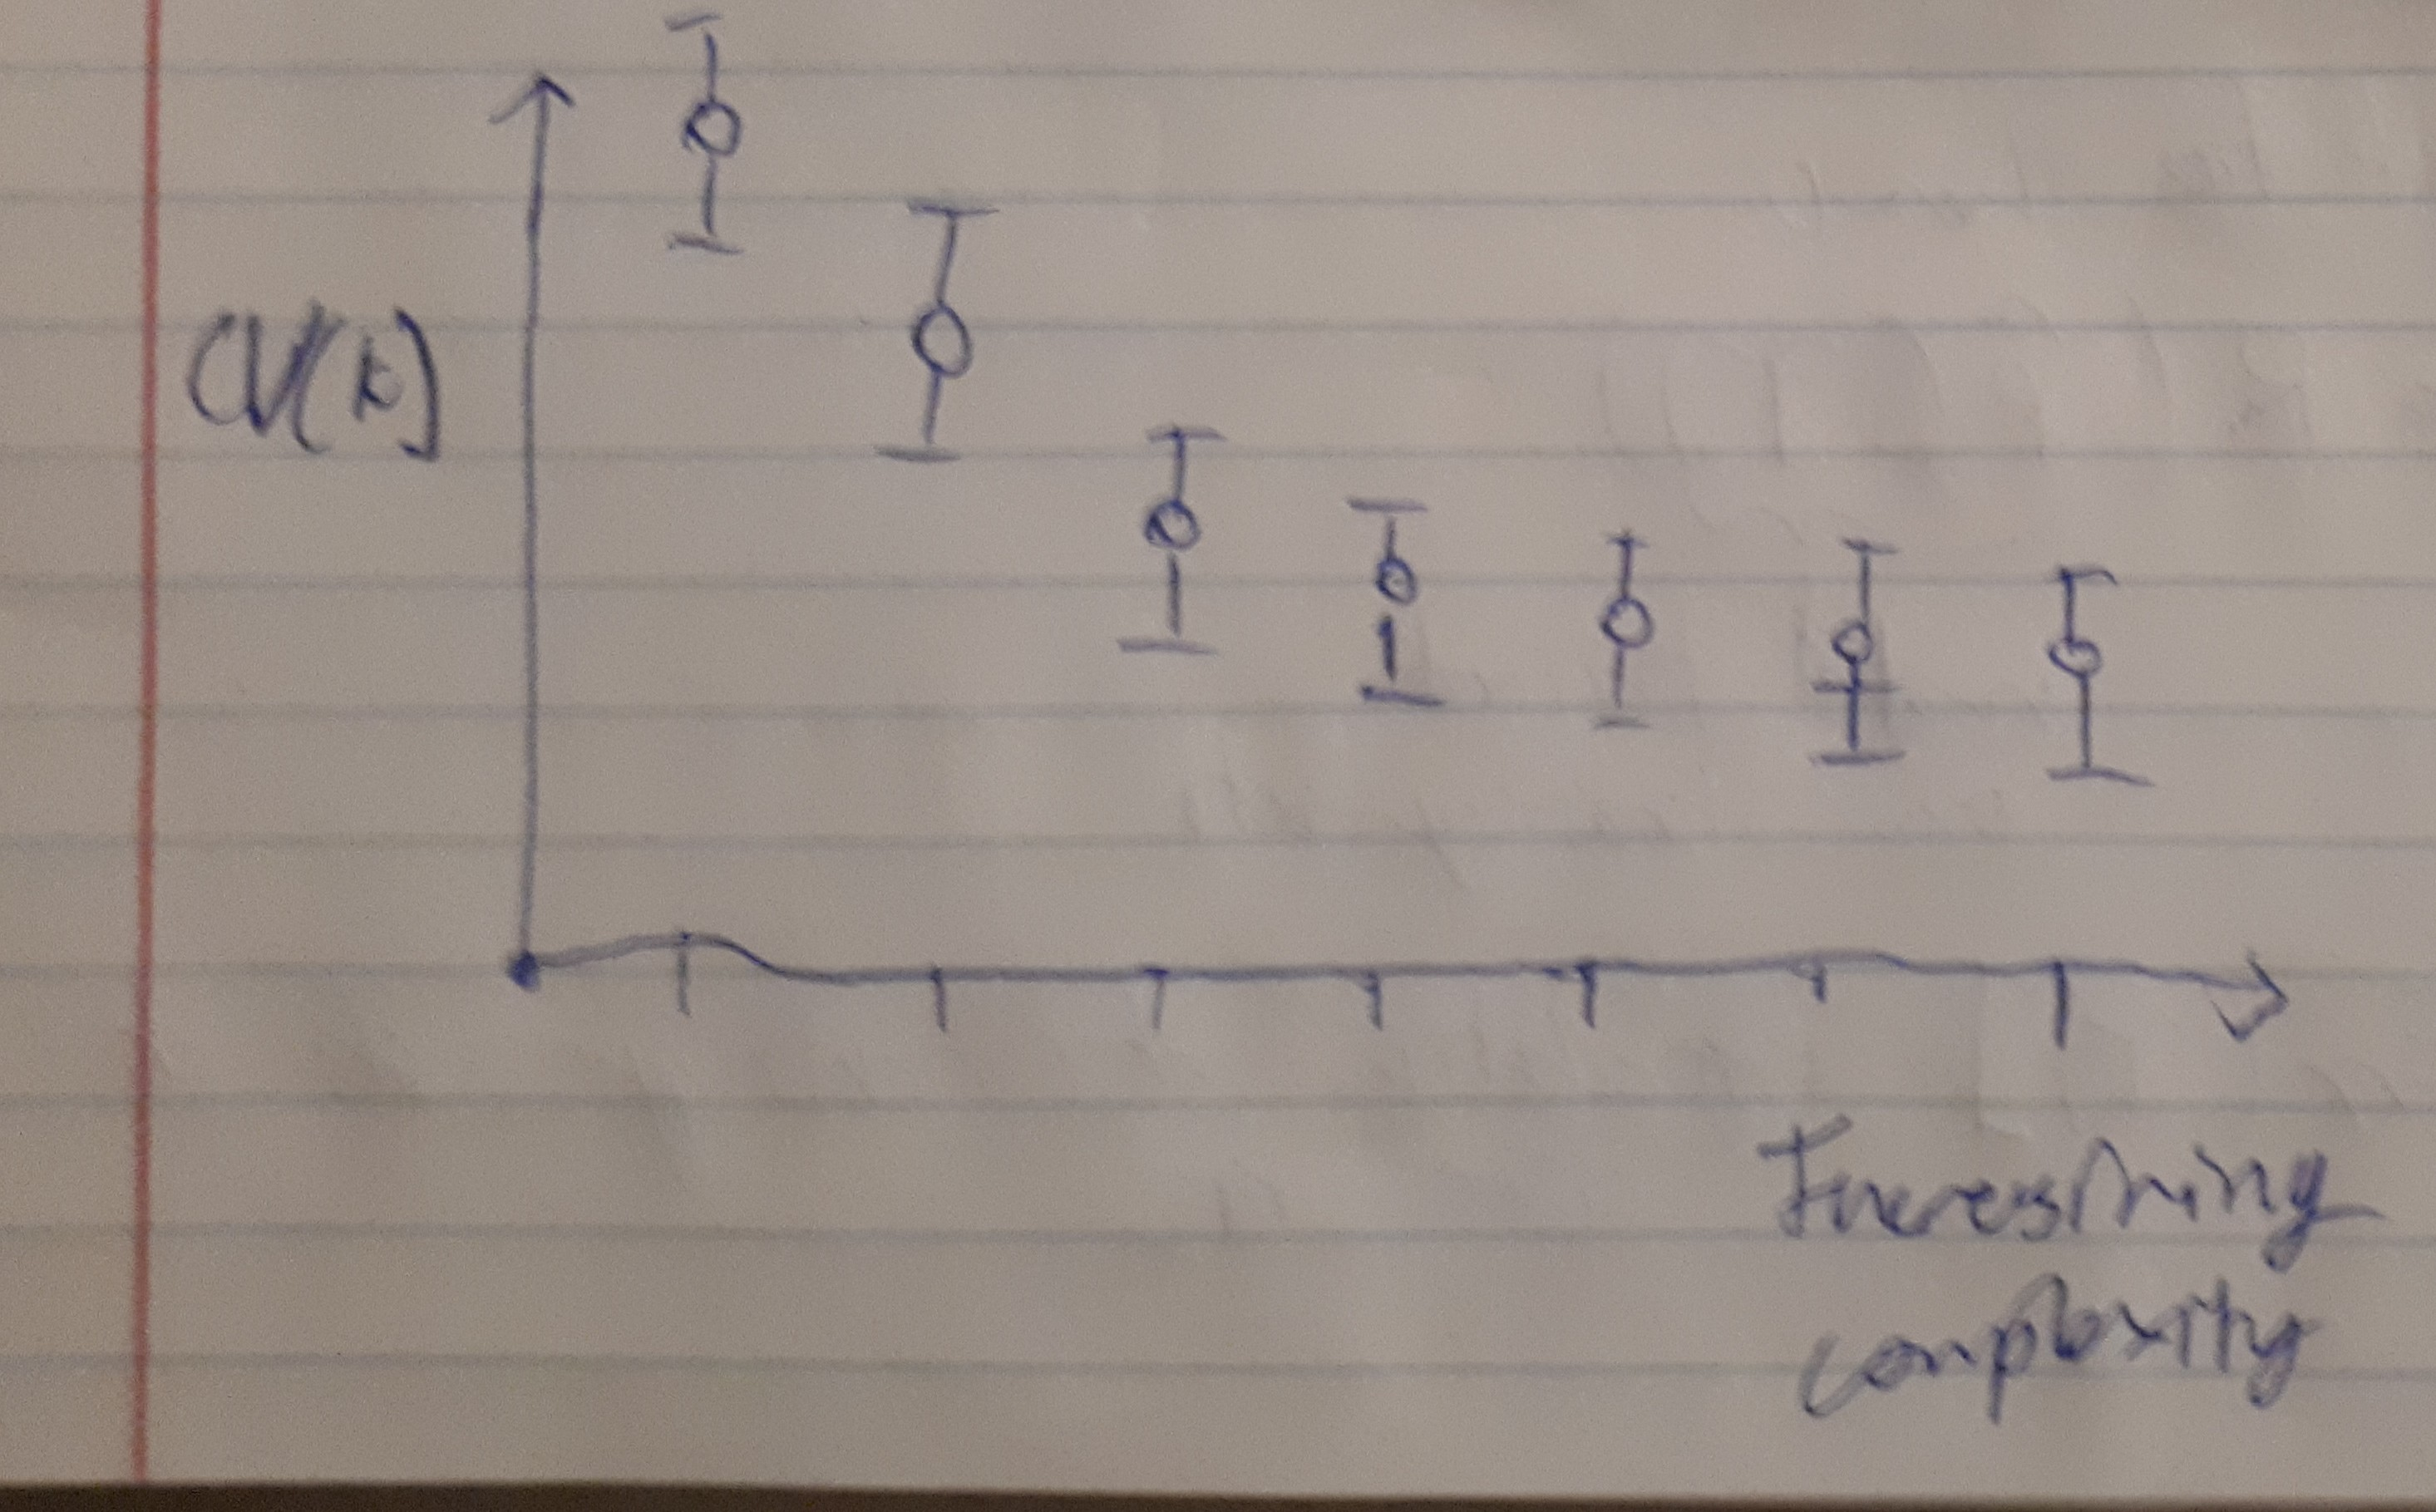
\includegraphics[width = 0.7\textwidth]{11_16_P01.jpg}
\end{center}

As we increase complexity (ie increase $\frac{1}{\la}$ in ridge regression or increase the number of components in PCA regression/forward stepwise), $CV(k)$ decreases. We can put error bars on $CV(k)$ by calculating the emperical standard deviation of $CV(k)$. This gives us the error bars in the plot. One may to choose $\la^*$ is to take the least complex model for which all the ``more complex'' models have $CV(k)$ within one standard error. We then fit a model using the full data and this chosen value of $\la^*$. 

\subsection{Leave one out cross validation}
Returning to the idea of taking $k$ large, we can set $k=n$. This is nice because then $CV(k)$ is unbiased for $\text{Err}_{\frac{n-1}{n}}$ which should be close to $\text{Err}_{n}$. When $k=n$ each fold is a single data point and so we set $J(i)=\{i\}$. There are two issues:
\begin{itemize}
    \item This may by computationally challenging we have to fit $n$ models for each model fitting procedure.
    \item The variance of $CV(n)$ may be larger than when $k=5$ or $k=10$ (this is still disputed).
\end{itemize}
In ordinary least squares we have computational tricks that means that $n$-fold cross validation can be done quickly. Suppose that we are using the model $y=X\beta+\eps$ to fit $\wh{\beta}$. That is $\wh{\beta}=(X^TX)^{-1}X^Ty$ and \[\wh{y}=X\wh{\beta}=X(X^TX)^{-1}X^Ty=Hy.\]
If we let $H_{ii}$ be the leverage scores of the model (the diagonal entries of $H$), then we have previously seen that 
\[\wh{y}_i = H_{ii}y+(1-H_{ii})\wh{y}_{- i}, \]
where $\wh{y}_{- i} = x_i^T\wh{\beta}^{- i}$ is the prediction for $y_i$ given only $(X_{- i}, y_{- i})$. Thus we have 
\[\wh{y}_{- i} = \frac{y_i}{1-H_{ii}}\wh{y}_i - \frac{H_{ii}}{1-H_{ii}}y_i. \]
And so
\[y_i - \wh{y}_{- i} = \frac{y_i-\wh{y}_i}{1-H_ii}. \]
Thus for fitting $\wh{\beta} = (X^TX)^{-1}X$ we have
\[CV(n) = \frac{1}{n}\sum_{i=1}^n \frac{(y_i-\wh{y}_i)^2}{(1-H_{ii})^2}, \]
under square error loss. This method can be used when $\la$ determines $X$ and then $\wh{\beta}$ is given by ordinary least square regression.

In general, computing $\wh{\beta}^{-i}$ can sometimes be easy and sometimes very hard. Suppose that instead of squared error we fit a model with the more general loss 
\[L_n(b) = \frac{1}{n}\sum_{i=1}^n l(y_i-x_i^Tb).\]
A very effective stratergy is to approximate $L_n$ with a quadratic at $\wh{\beta} =\amin_b L_n(b)$, then remove the $i^{th}$ term and choose $\wh{\beta}^{-i}_{\text{quad}}$ to be the value which minimizes the approximation. More specifically we have
\[L_n(b) \approx L_n(\wh{\beta}) -\frac{1}{n}\sum_{i=1}^n l'(y_i-x_i^T\wh{\beta}_i)x_i^T(b-\wh{\beta})+\frac{1}{2n}\sum_{i=1}^n (b-\wh{\beta})^Tl''(y_i-x_i^T\wh{\beta})x_ix_i^T(b-\wh{\beta}).\] 
Define $\wh{\eps}_i = y_i-x_i^T\wh{\beta}$, then 
\begin{align*}
    L_{-i}(b) &= \frac{1}{n-1}\sum_{j \neq i}L_j(y_j-x_j^Tb)\\
    &\approx \frac{1}{n-1}\sum_{j \neq i}L_j(\wh{\eps}_j)-\frac{1}{n-1}\sum_{j \neq i}l'(\wh{\eps}_j)x_i^T(b-\wh{\beta})+\frac{1}{2(n-1)}\sum_{j \neq i}(b-\wh{\beta})^Tl''(\wh{\eps}_j)x_ix_i^T(b-\wh{\beta})\\
    &= c+g_{-i}^T b + \frac{1}{2}b^TA_{-i}b,
\end{align*}
where
\[g_{-i} = -\frac{1}{n-1}\sum_{j\neq i}\left(l'(\wh{\eps}_j)x_j+l''(\wh{\eps}_j)x_jx_j^T\wh{\beta}\right),\]
and
\[A_{-i} = \frac{1}{n-1}\sum_{j\neq i} l''(\wh{\eps}_j)x_jx_j^T. \]
The minimizer of the quadratic approximation is
\[ \wh{\beta}^{-i}_{\text{quad}} = -A^{-1}_{-i}g_{-i}.\]
Note that the matrix $A_{-i}$ differs from the Hessian of $L_n(\wh{\beta})$ by a rank one update. Thus inverting $A_{-i}$ can be done quickly provided that we have stored the inverse Hessian. 
\section{Permuation testing}
We will leverage the fact that if two random variables have no relationship (ie $X_i$ and $Y_i$ are independent), then 
\[(X_i,Y_i)_{i=1}^n \stackrel{\text{dist}}{=} (X_i, Y_{\pi(i)})_{i=1}^n, \]
where $\pi : [n] \to [n]$ is a permutation of $[n]=\{1,2,\ldots,n\}$. Thus under independence, any statistic $T_n = T((X_i,Y_i)_{i=1}^n)$ should have the same distribution under permutations i.e.
\[T_n  \stackrel{\text{dist}}{=}  T((X_i,Y_{\pi(i)})_{i=1}^n).\]
\begin{defn}
    Let $S_1,\ldots, S_N$ be real values statistics and define the \emph{emprical CDF} of $s_i$ to be
    \[F_N(t) = \frac{1}{N}\sum_{i=1}^N \mathbb{I}(S_i \le t), \]
    where $\mathbb{I}(S_i \le t)$ is 1 if $S_i \le t$ and 0 otherwise. 
\end{defn}
The function $F_N$ is a step function that looks something like this:

\begin{center}
    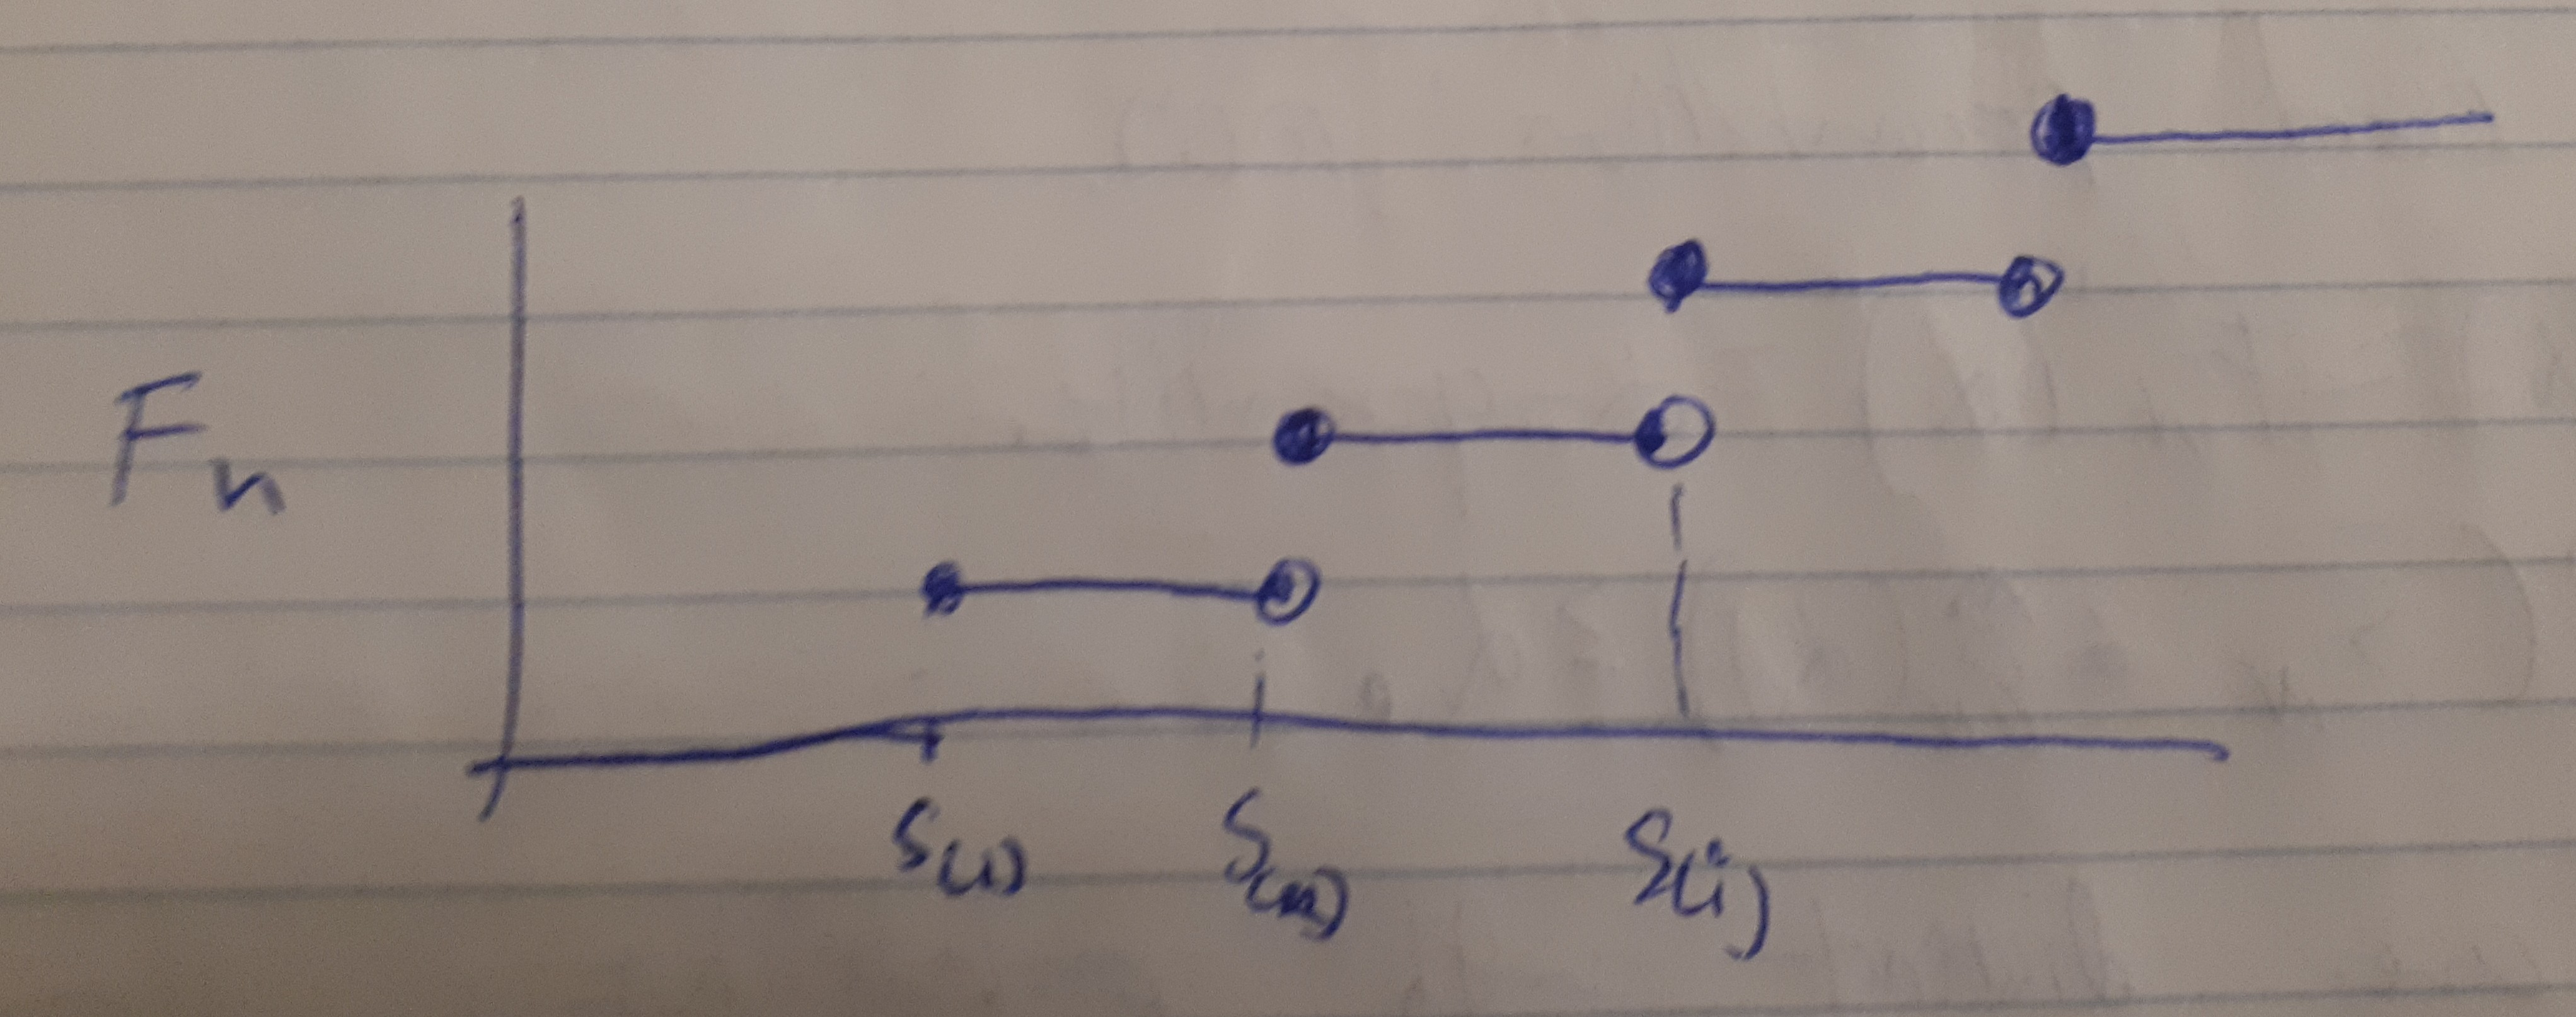
\includegraphics[width = 0.7\textwidth]{11_16_P02.jpg}
\end{center}

Note that $F_N(t)$ is right continuous.
\begin{defn}
    With $S_i$ as before define the \emph{quartile function} to be
    \[\wh{q}_N(\al)=F_N^{-1}(\al) = \inf\{t \in \R : F_N(t) \ge \al\}.\]
\end{defn}
The qunatile function looks like this:
\begin{center}
    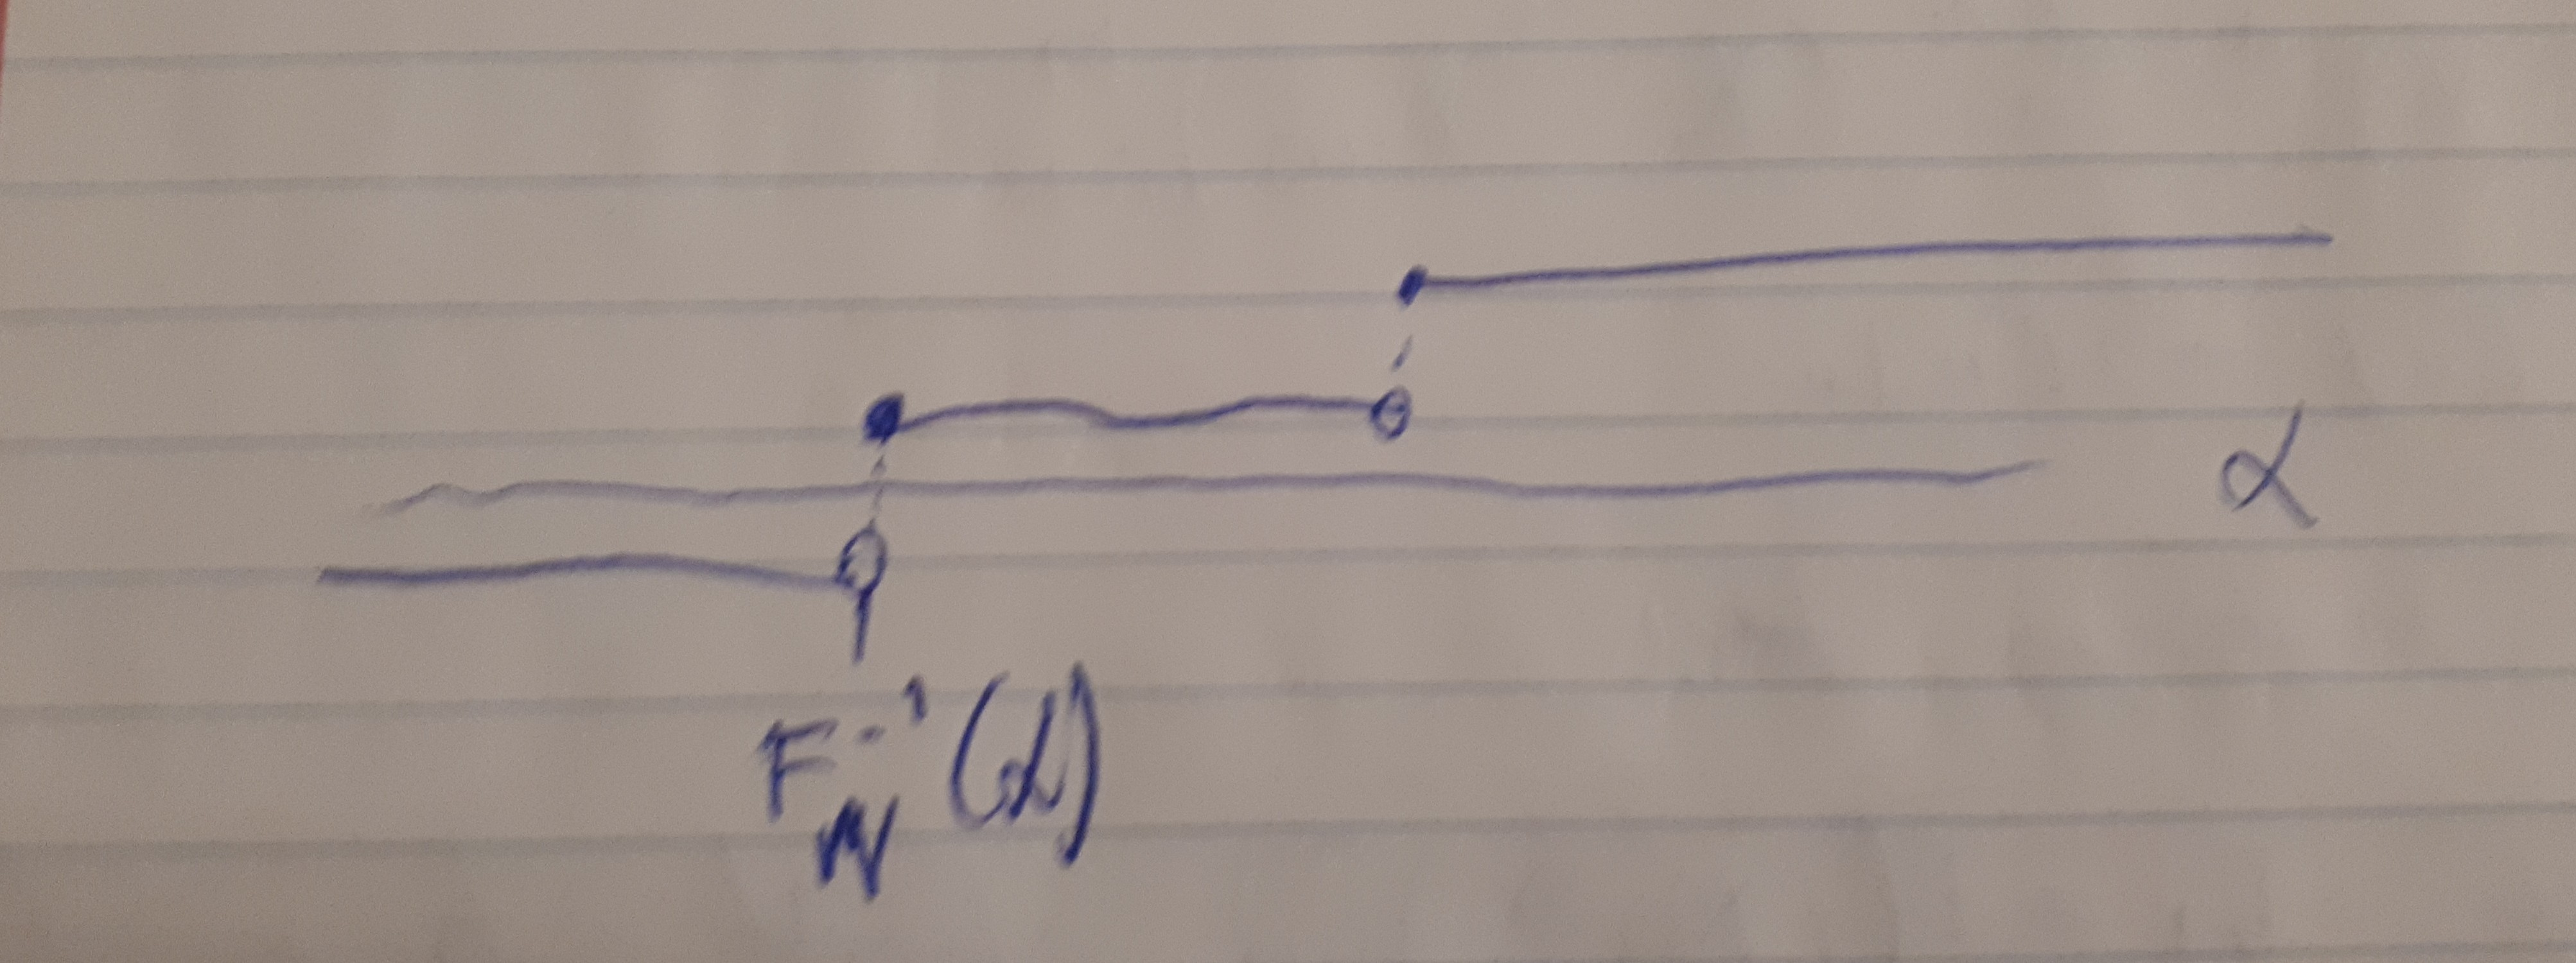
\includegraphics[width = 0.7\textwidth]{11_16_P03.jpg}
\end{center}
Note that $F_N(F_N^{-1}(\al)) \ge \al$ for all $\al$ and that $F_N^{-1}(i/N) = S_{(i)}$ if 
\[S_{(1)} < S_{(2)} < \ldots < S_{(N)}.\]
\begin{thrm}
    Suppose that the statistics $S_1,\ldots, S_N$ are exchangable and so that for all permutations $\pi$
    \[(S_1,\ldots, S_N) \stackrel{\text{dist}}{=} (S_{\pi(1)},\ldots S_{\pi(N)}).\]
    Let $\wh{q}_N = F_N^{-1}$ be the quartile function. Then 
    \[ \Pa(S_N \le \wh{q}_N(\al)) \ge \al,\]
    for all $\al$. If $S_1,\ldots, S_N$ are all distinct with probability one, then
    \[\Pa(S_N \le \wh{q}_N(\al)) \le \al + \frac{1}{N}. \]
\end{thrm}
\begin{proof}
    Note that for all $i$, $\Pa(s_i \le \wh{q}_N(\al)) = \Pa(S_N \le \wh{q}_N(\al))$ by exchangability. Thus
    \begin{align*}
        \E[F_N(\wh{q}_N(\al))]&=\frac{1}{N}\sum_{i=1}^N \Pa(S_i \le \wh{q}_N(\al))\\
        &=\Pa(S_N \le \wh{q}_N(\al)).
    \end{align*}
    We also know that $F_N(\wh{q}_N(\al)) \ge \al$ and so 
    \[\Pa(S_N \le \wh{q}_N(\al)) = \E[F_N(\wh{q}_N(\al))] \ge \al. \]
    And if $S_i$ are distinct then the size of the jumps in $F_N$ are exactly $\frac{1}{N}$ and so 
    \[F_N(\wh{q}_N(\al)) \le \al + \frac{1}{N}. \]
    This thus implies
    \[\Pa(S_N \le \wh{q}_N(\al)) = \E[F_N(\wh{q}_N(\al))] \le \al+\frac{1}{N}.\] 
\end{proof}
The upshot is that we should think of $\Pa(S_N \le \wh{q}_N(\al))$ as being equal to $\al$ but there is some error due to discretization. The error has size $\le \frac{1}{N}$. 

Note that as a consequence we have $\Pa(S_N > \wh{q}_N(\al)) \le \al$ since
\[\Pa(S_N > \wh{q}_N(\al)) = 1-\Pa(S_N \le \wh{q}_N(\al)) \le 1-(1-\al)=\al. \]
\begin{ex}
    Say we have i.i.d data $(X_i,Y_i)$ and we want to test the null $H_0 : X_i \ind Y_i$. Under the null, $(X_i,Y_i) \stackrel{\text{dist}}{=} (X_i,Y_{\pi(i)})$. We can fit $\wh{\beta}=(X^TX)^{-1}X^TY$ and $\wh{\beta}_\pi = (X^TX)^{-1}X^TY_\pi$ where
    \[Y_\pi = \begin{bmatrix}
        Y_{\pi(1)}\\ \vdots \\ Y_{\pi(n)}
    \end{bmatrix}.\]
    Suppose we do this for $m-1$ random permuations. Set $S_m = \norm{\wh{\beta}}_2^2$ (although we could use \underline{any} function of $\wh{\beta}$) and $S_i = \norm{\wh{\beta}_{\pi}}_2^2$. We can then reject $H_0$ if 
    \[S_m \ge \text{ Quantile}_{1-\al}(S_{\pi_i},S_m).\]
    This test will have level $\al$.
\end{ex}
\end{document}